\begin{figure}
    \centering
    \begin{tabular}{c c | c c}
        \multicolumn{2}{c}{Frame 1} & \multicolumn{2}{c}{Frame 5} \\
        %\hline
        %  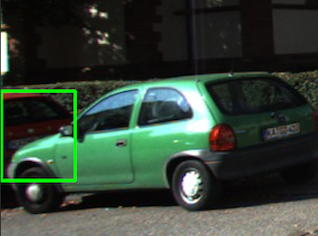
\includegraphics[width=0.2\textwidth]{figures/method/multiframe/ex1/rgb-1.png}
        % &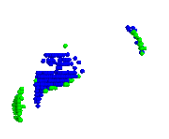
\includegraphics[width=0.2\textwidth]{figures/method/multiframe/ex1/pcd-1.png} &
        %  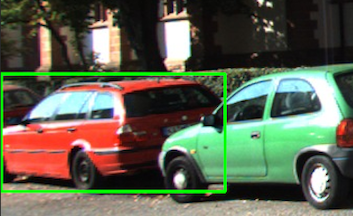
\includegraphics[width=0.2\textwidth]{figures/method/multiframe/ex1/rgb-5.png}
        % &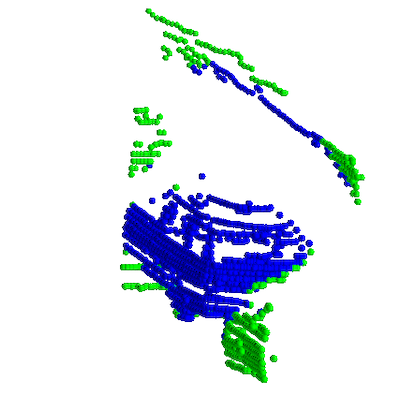
\includegraphics[width=0.2\textwidth]{figures/method/multiframe/ex1/pcd-5-1.png} \\
         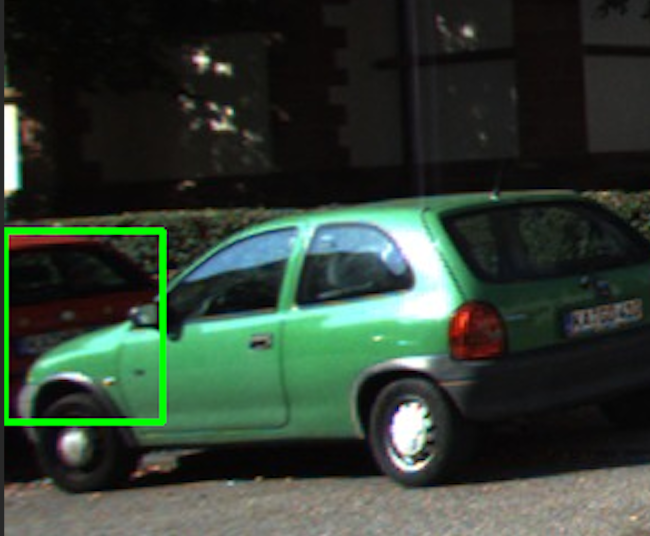
\includegraphics[height=0.16\textwidth]{figures/method/multiframe/ex3/rgb-1.png}
        &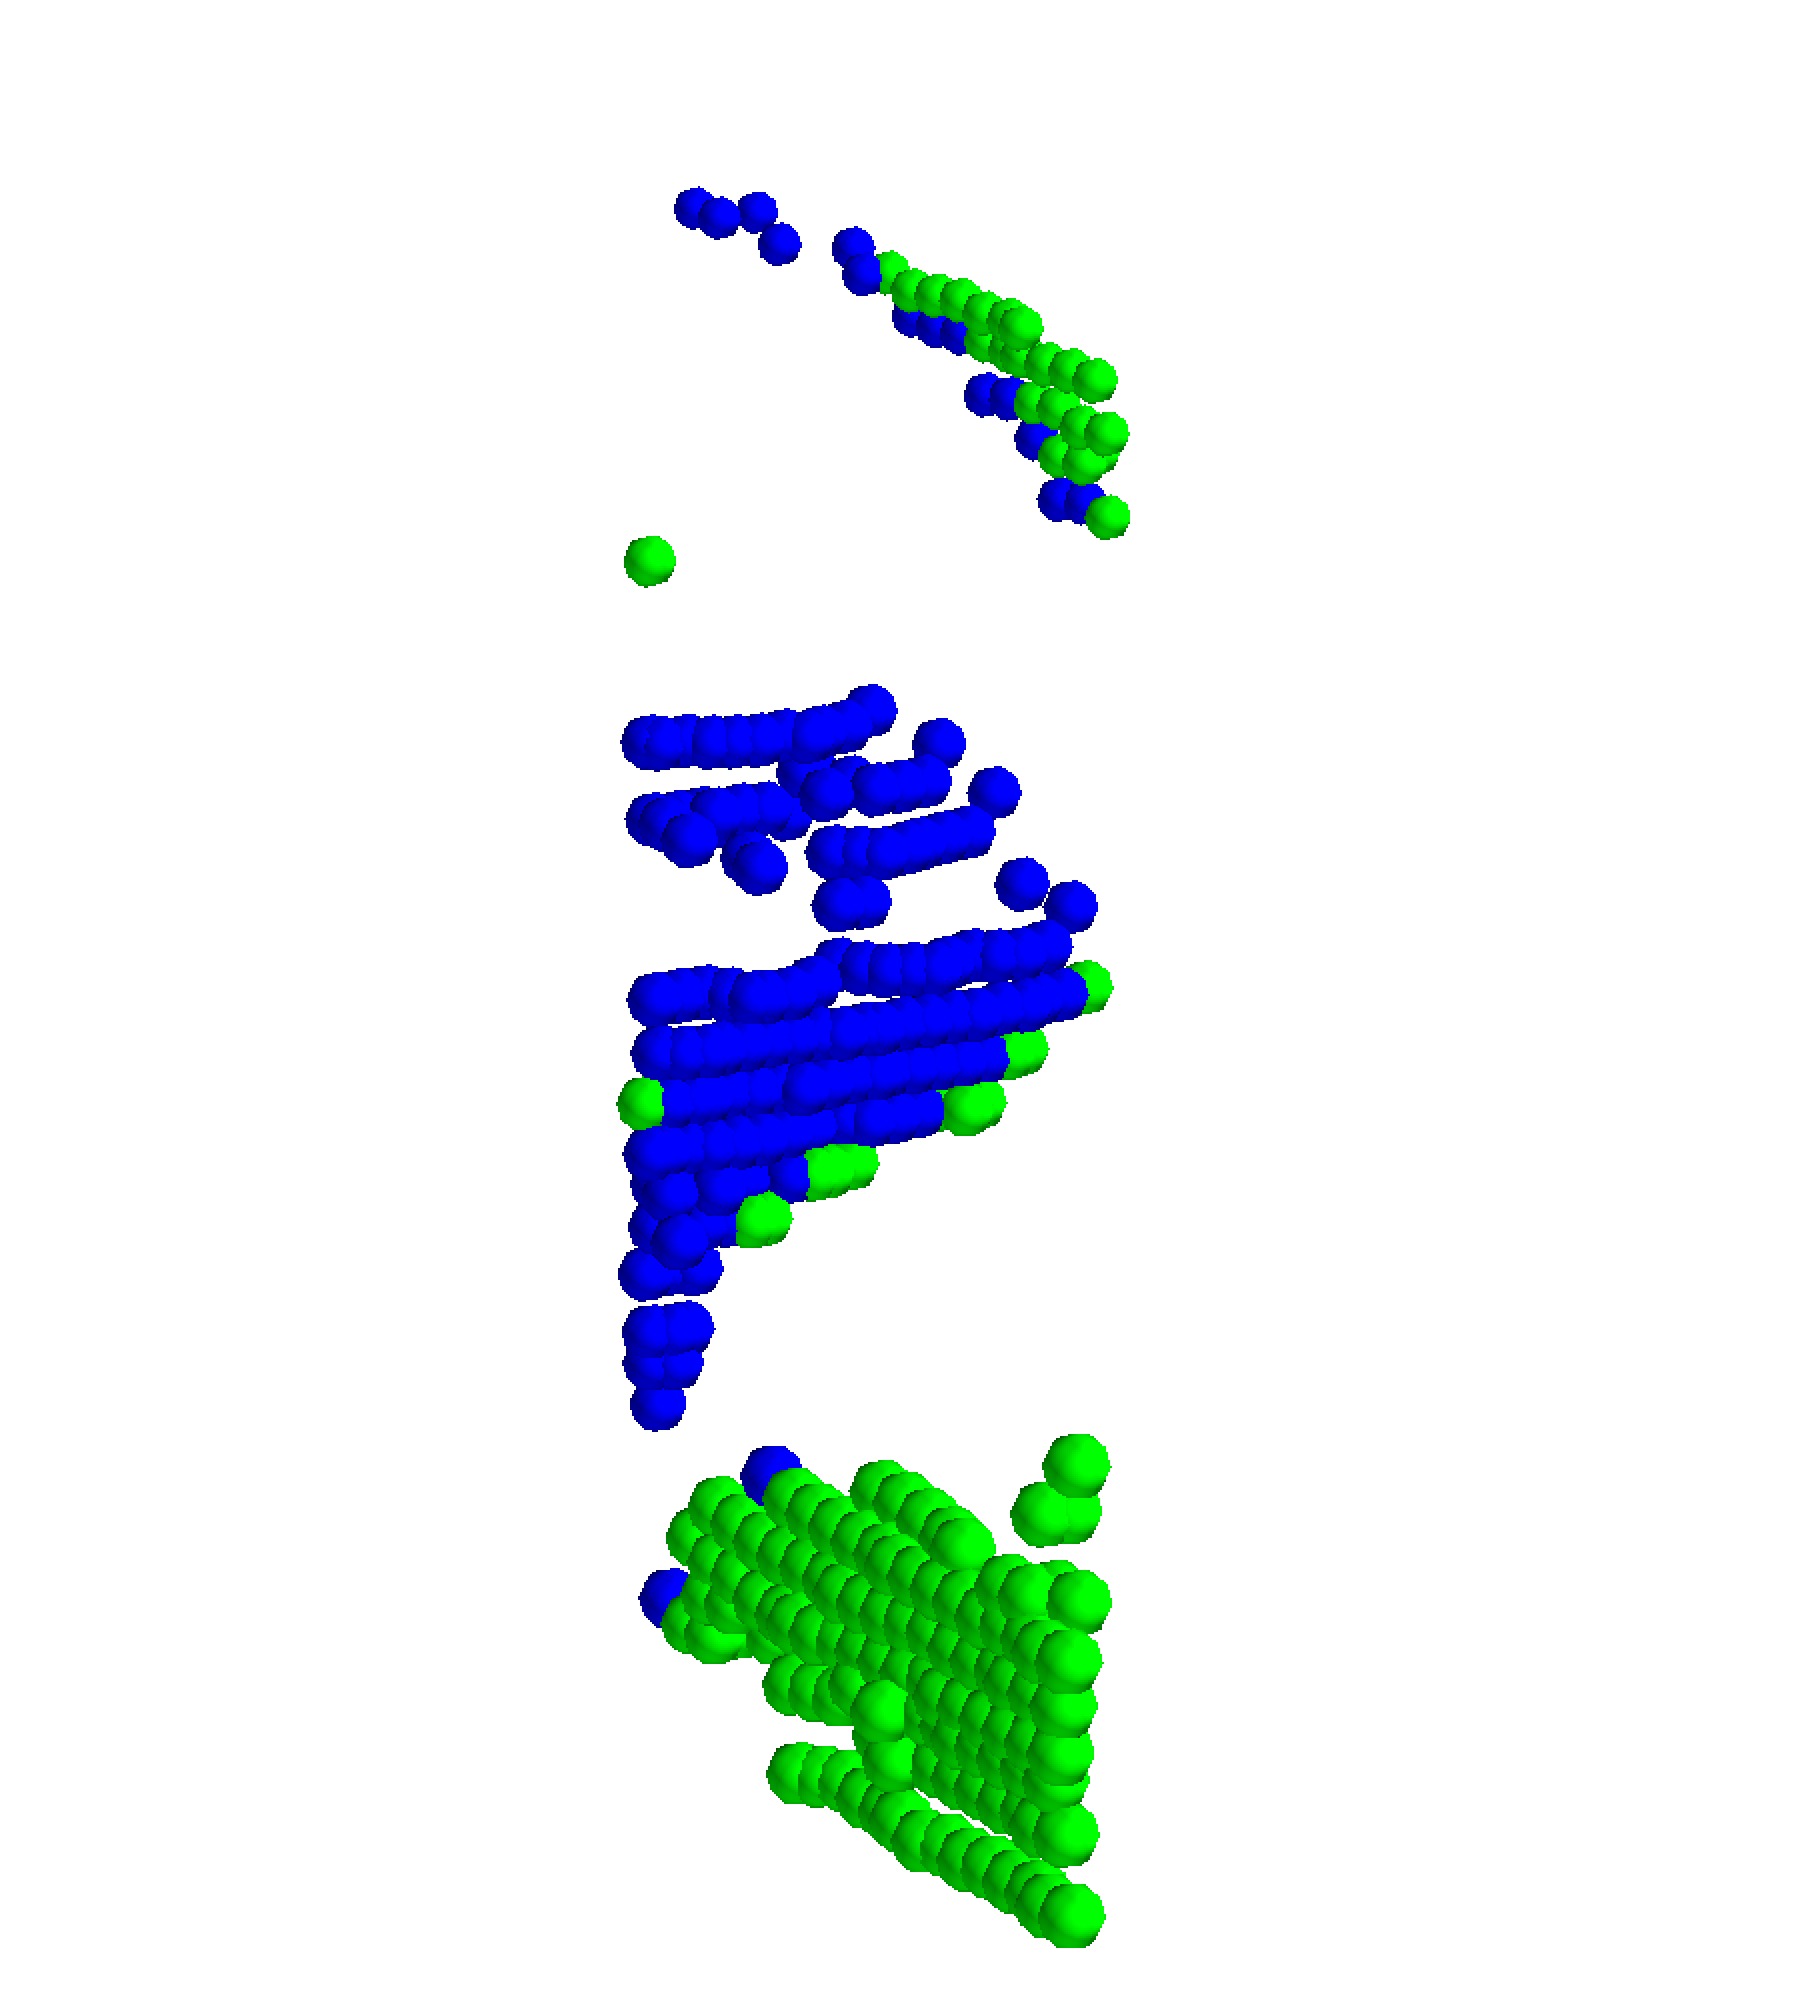
\includegraphics[width=0.15\textwidth]{figures/method/multiframe/ex3/pcd-1.png} &
         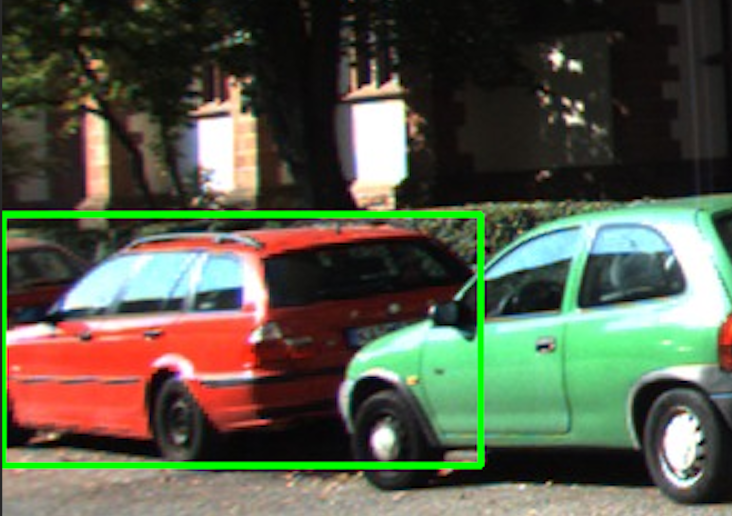
\includegraphics[height=0.16\textwidth]{figures/method/multiframe/ex3/rgb-5.png}
        &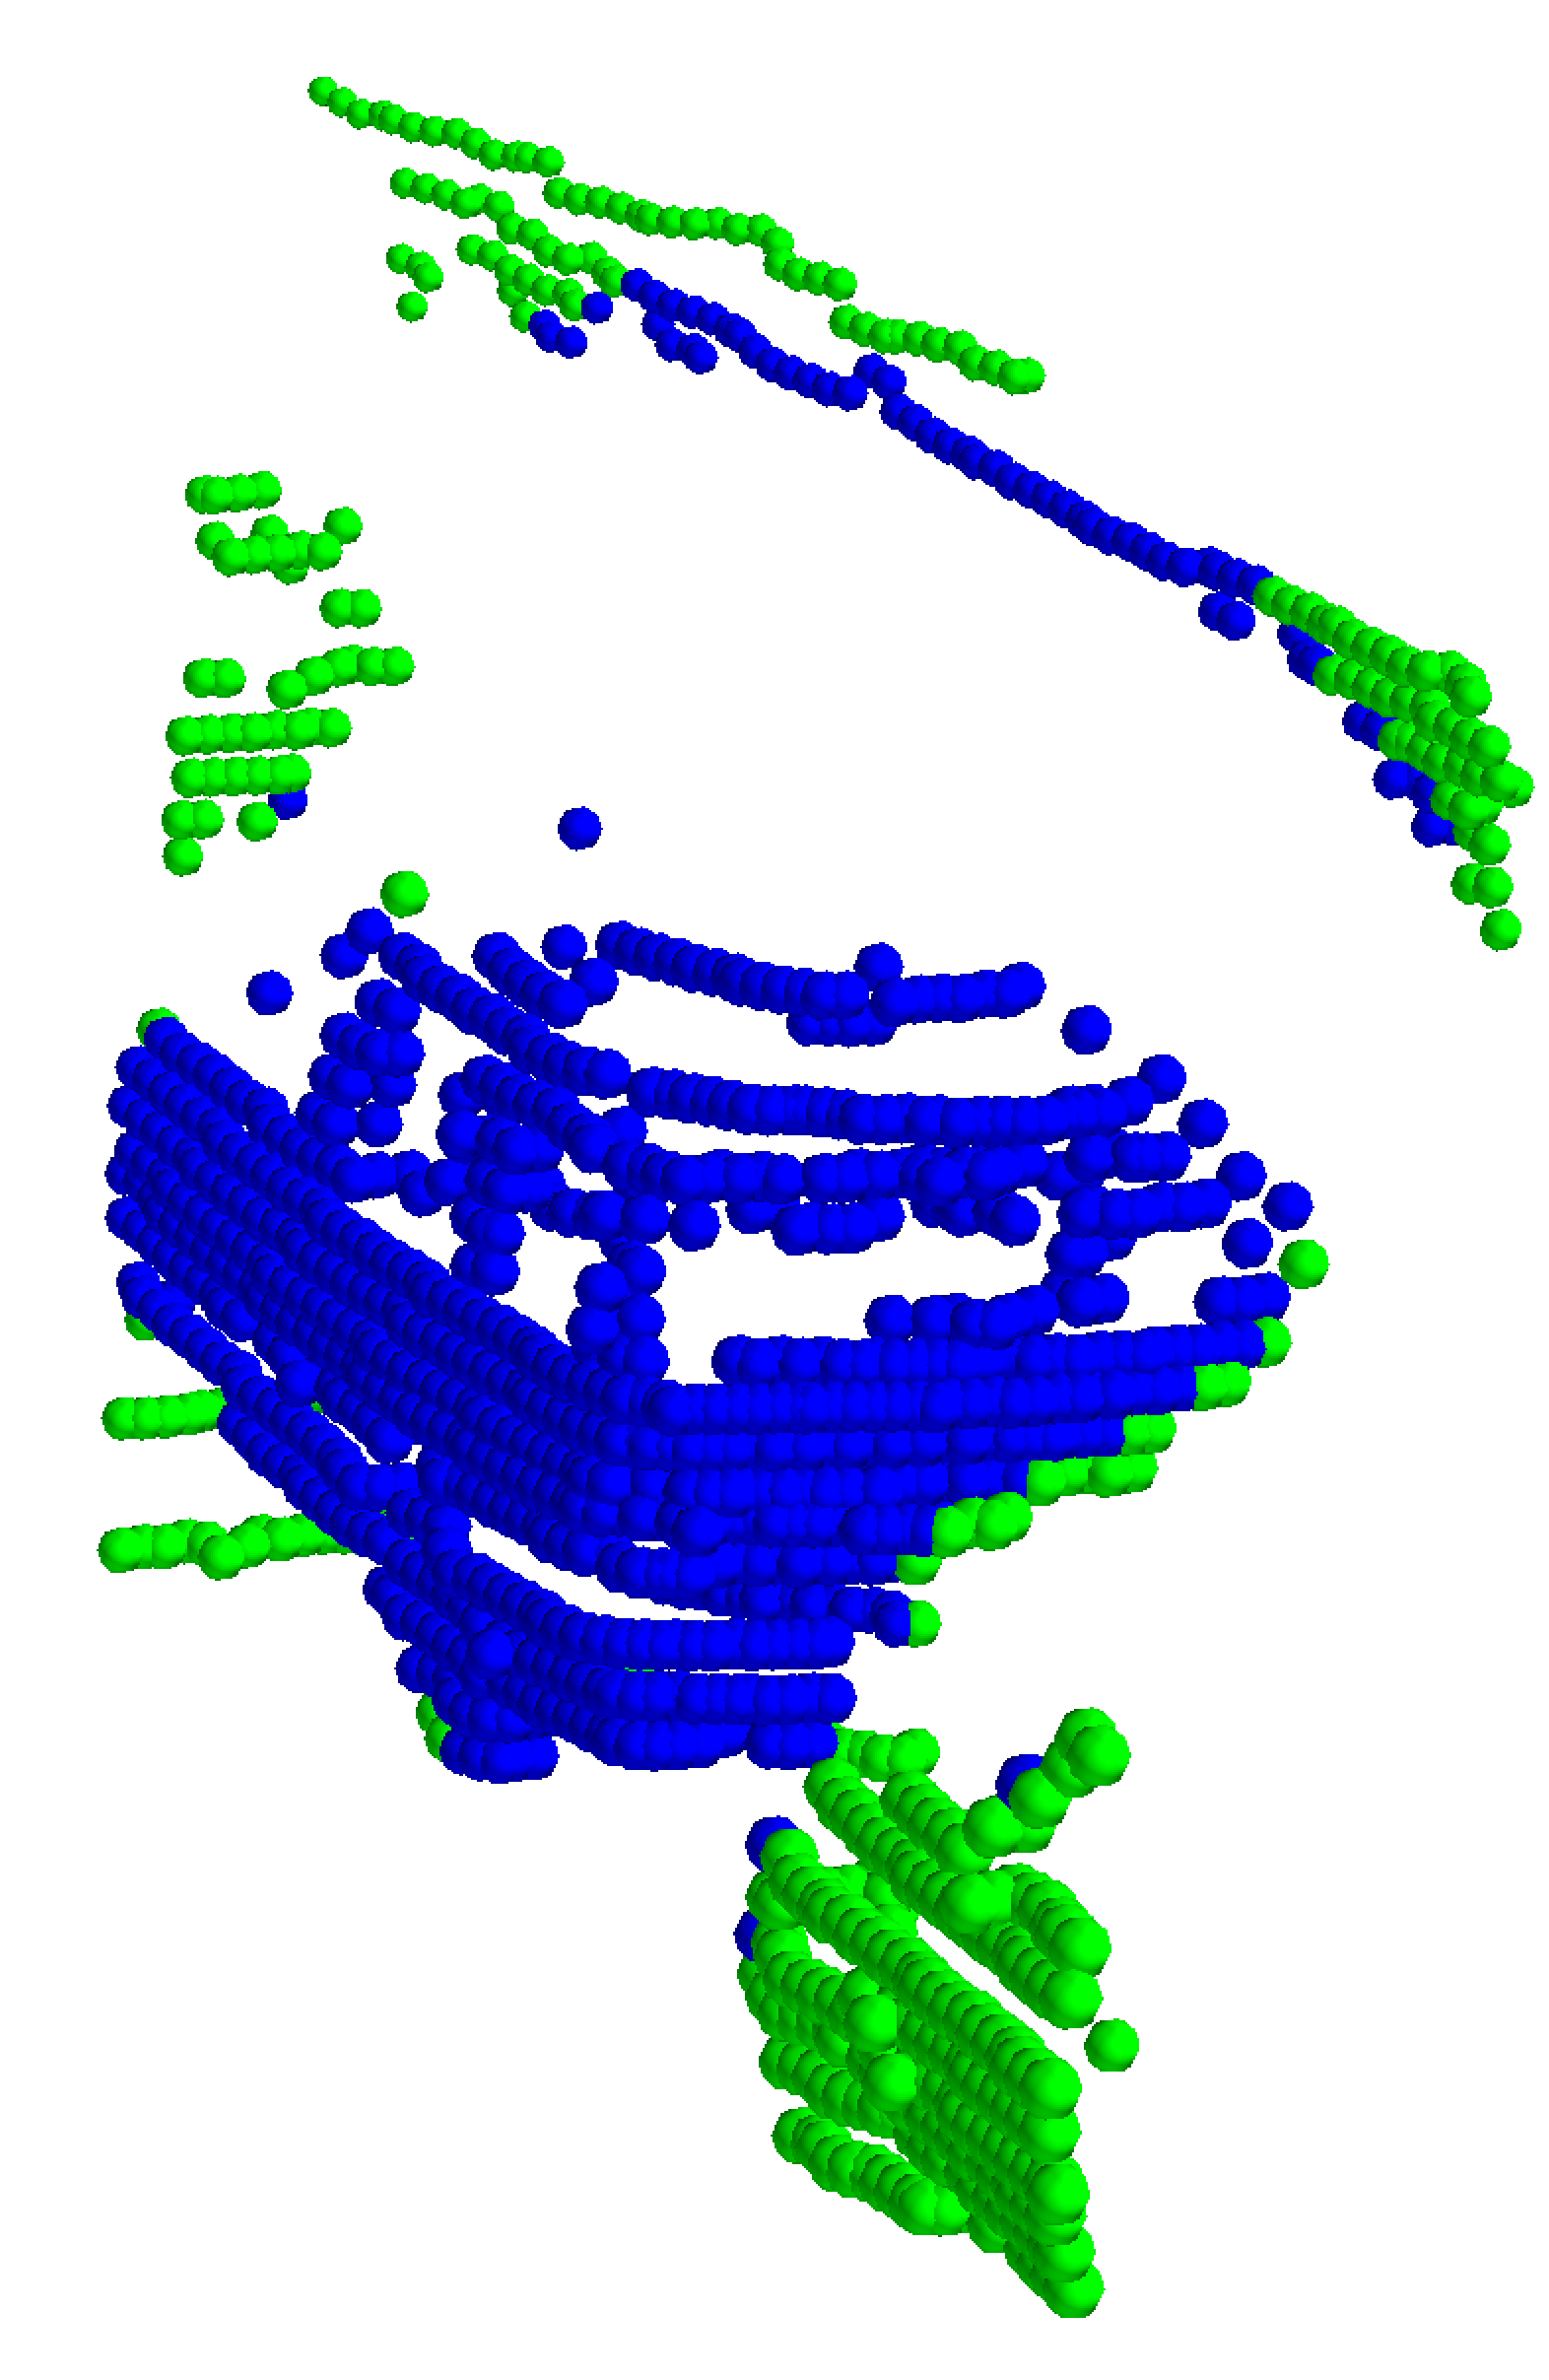
\includegraphics[height=0.2\textwidth]{figures/method/multiframe/ex3/pcd-5.png} \\
    \end{tabular}
    \caption{Two frames in a sequence of five, with a heavily occluded and truncated car in the first frame and a much better view of the same in the last.
    Multi-frame consistency allows the method to use clearer frames to interpret more difficult ones, which is particularly helpful in discovering the outliers.}\label{fig:multiframe_example}
    % On the left we see examples from the first frame of five where the car of interest is heavily occluded or truncated.
    % whereas in the last frame the vehicle is much better described by the point cloud allowing our method to more confidently fit and thus improve the difficult examples through consistency}
\end{figure}